\documentclass[aspectratio=169,12pt]{beamer}
\usetheme{Madrid}
\usecolortheme{dolphin}
\usefonttheme{professionalfonts}
\setbeamertemplate{navigation symbols}{}
\setbeamertemplate{footline}{}

\usepackage[T1]{fontenc}
\usepackage[utf8]{inputenc}
\usepackage{graphicx}
\usepackage{amsmath,amssymb}
\usepackage{hyperref}
\usepackage[normalem]{ulem}
\usepackage{physics}

\usepackage{tikz}

\begin{document}

\title[Chapter 2]{Chapter 2: Vectors, qubit and superposition}
\author{JAMOTTE Maxime, SCHOONEN Cédric}
\institute{Digital Learning Hub}
\date{}

\begin{frame}
  \titlepage
\end{frame}

\begin{frame}{Chapter 2 objectives}
  \begin{enumerate}
    \item Vectors\\~\\
    %\item Dot product\\~\\
    \item Qubit, superposition of states and vectors\\~\\
    \item Measuring the state of a qubit
  \end{enumerate}
\end{frame}

\begin{frame}{Vectors}
  {%
    \setbeamercolor{itemize/enumerate body}{fg=gray!60}
    \setbeamercolor{itemize item}{fg=gray!60}
    \setbeamercolor{alerted text}{fg=black}
    \begin{columns}[T]
      \begin{column}{0.55\textwidth}
        \begin{itemize}[<+-| alert@+>]
          \setlength{\itemsep}{0.6em}
          \item Definition of a vector
          \item Addition of vectors
          \item Multiplication of a vector by a constant
        \end{itemize}
        \bigskip
        \only<1>{\[
          \vec r = \begin{pmatrix} a \\ b \end{pmatrix}
        \]}
        \only<2>{\[
          \vec r + \vec p = 
          \begin{pmatrix} a \\ b \end{pmatrix} +
          \begin{pmatrix} c \\ d \end{pmatrix} =
          \begin{pmatrix} a+c \\ b+d \end{pmatrix}
        \]}
        \only<3>{\[
          \lambda \begin{pmatrix} a \\ b \end{pmatrix} =
          \begin{pmatrix} \lambda a \\ \lambda b \end{pmatrix}
        \]}
      \end{column}
      \begin{column}{0.4\textwidth}
        \centering
        \only<1>{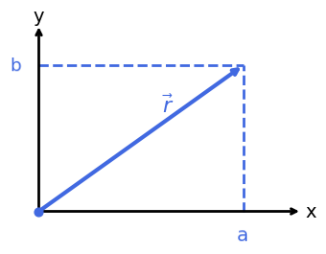
\includegraphics[width=\linewidth]{../figures/math/vecteur.png}}
        \only<2>{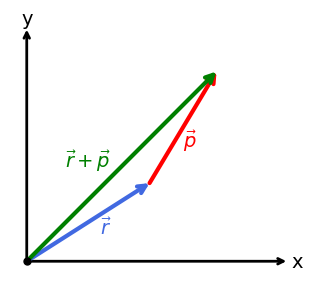
\includegraphics[width=\linewidth]{../figures/math/add_vecteurs.png}}
        \only<3->{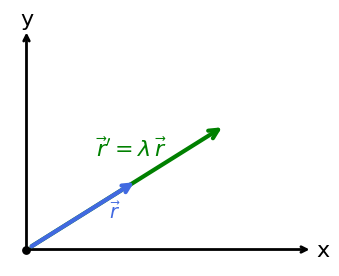
\includegraphics[width=\linewidth]{../figures/math/multiplication_nombre.png}}
      \end{column}
    \end{columns}
  }
\end{frame}

\begin{frame}{Qubit}
  \begin{itemize}[<+->]
    \setlength{\itemsep}{0.6em}
    %\item Electron around the nucleus: infinity of possible positions.
    \item The electron passes through the top ($T$) and bottom ($B$) slits at the same time.% $\ket{\psi_e^{}} = \alpha \ket{T} + \beta \ket{B}$.
      \only<1->{%
        \vspace{0.5em}
        \begin{center}
          \begin{minipage}{0.42\textwidth}
            \centering
            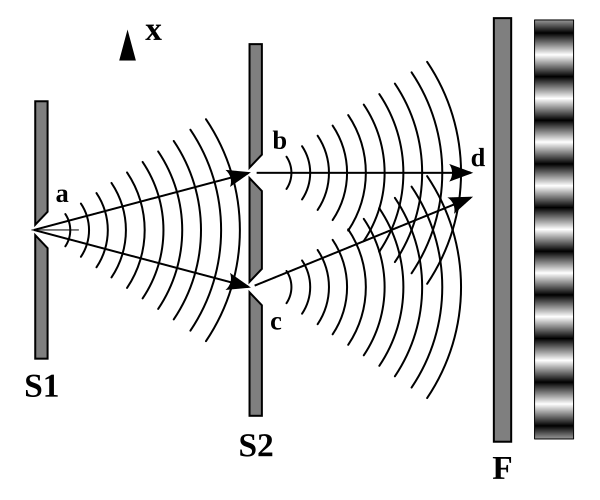
\includegraphics[width=0.6\linewidth]{../figures/intro/fente_Young.png}
          \end{minipage}\hfill
          \begin{minipage}{0.42\textwidth}
            \centering
            \only<2->{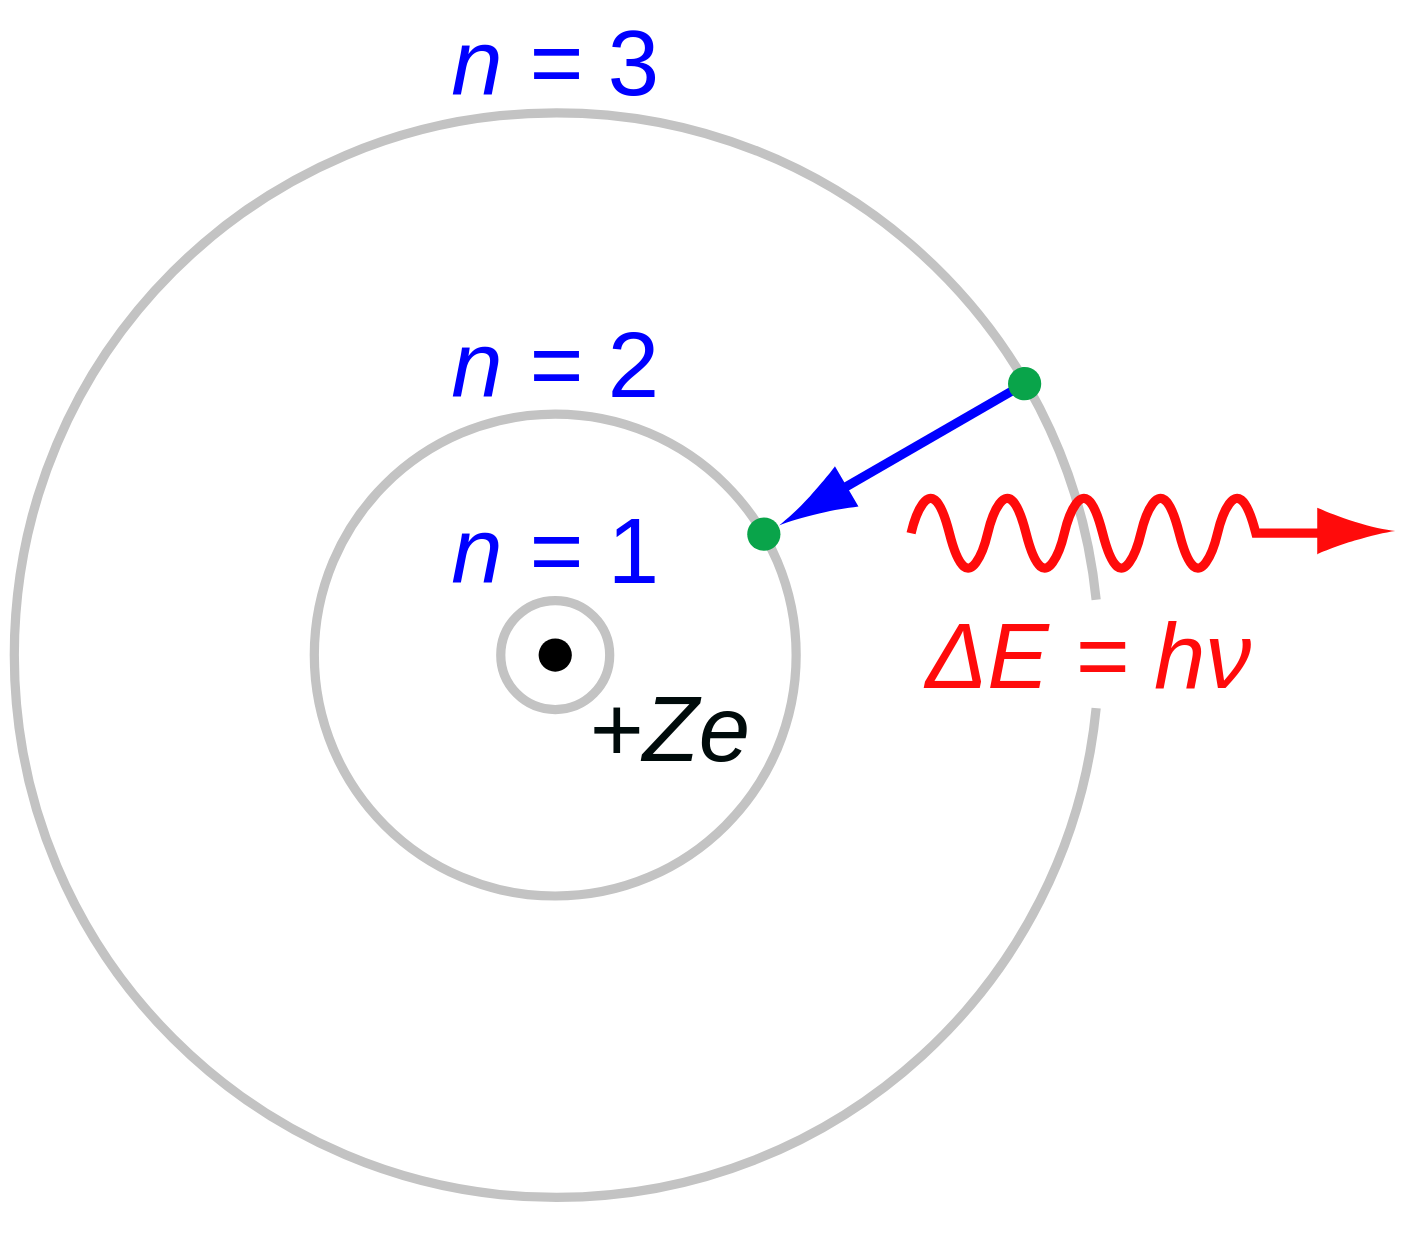
\includegraphics[width=0.6\linewidth]{../figures/intro/bohr_model.png}}
          \end{minipage}
        \end{center}
      }
    \item Some physical systems have discrete energy levels (instead of position).
    \item \textbf{Qubit} (= quantum bit) = two-level quantum system, labelled $\ket 0$ and $\ket 1$.
  \end{itemize}
\end{frame}

\begin{frame}{Superposition of states and vectors}
  \begin{columns}[T]
    \begin{column}{0.65\textwidth}
      \begin{itemize}[<+->]
        \item A qubit can be in $\ket 0$, $\ket 1$ or any \textbf{superposition} of both: $\alpha \ket 0 + \beta \ket 1$.
        \item Superposition = linear combination of states.
        % \item \textbf{Postulate}: quantum states form a vector space (Hilbert space). A linear combination of states is also a state.
        \item The superposed state $\ket {\psi} = \alpha \ket 0 + \beta \ket 1$, is written $\begin{pmatrix} \alpha \\ \beta \end{pmatrix}$,\\~\\
        \item Each \textbf{qubit} is identifiable with the \textbf{direction} of a vector.
        \item $\ket{0}$ and $-\ket{0}$ are the same quantum state.
        %\item Probabilités de mesure : $P(\ket 0)=|\alpha|^2$, $P(\ket 1)=|\beta|^2$,
        %$$ \Longrightarrow  |\alpha|^2 + |\beta|^2 = 1$$
      \end{itemize}
    \end{column}
    \begin{column}{0.35\textwidth}
      \vspace{2em}
      \centering
      $\ket 0 = \begin{pmatrix}1 \\ 0\end{pmatrix}$ and $\ket 1 = \begin{pmatrix}0 \\ 1\end{pmatrix}$\\~\\~\\
      \only<4->{
        \resizebox{0.8\textwidth}{!}{
        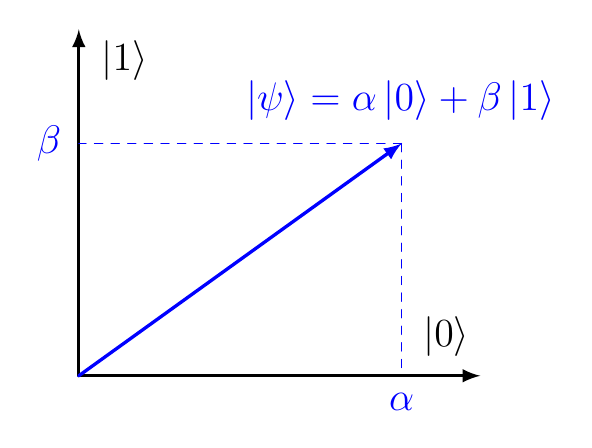
\begin{tikzpicture}[x=1cm,y=1cm,line cap=round,line join=round,>=latex]
        % Axes
        \draw[black,very thick,->] (0,0) -- (0,4.4);
        \draw[black,very thick,->] (0,0) -- (5.1,0);

        % State vector
        \draw[blue,very thick,->] (0,0) -- (4.1,2.95);
        \draw[blue,dashed] (4.1,2.95) -- (4.1,0);
        \draw[blue,dashed] (4.1,2.95) -- (0,2.95);

        % Labels
        \node[anchor=west,font=\Large] at (2.0,3.5) {\textcolor{blue}{$\ket{\psi} = \alpha \ket{0} + \beta \ket{1}$}};
        \node[anchor=north,text=blue,font=\Large] at (4.1,-0.1) {$\alpha$};
        \node[anchor=east,text=blue,font=\Large] at (-0.1,2.95) {$\beta$};

        \node[anchor=east,font=\Large] at (1.0,4.0) {$\ket{1}$};
        \node[anchor=west,font=\Large] at (4.25,0.5) {$\ket{0}$};
        \end{tikzpicture}
      }}
    \end{column}
  \end{columns}
\end{frame}


\begin{frame}{Measuring the state of a qubit}
  \begin{columns}[T]
    \begin{column}{0.65\textwidth}
      \begin{itemize}[<+->]
      \item To measure = to extract information\\~\\
      \item The interaction with the measurement apparatus destroys the superposition\\~\\
      \item The final state is then either $\ket 0$ or $\ket 1$.\\~\\
      \item Probability of measuring state $\ket 0$: $P(\ket 0)=|\alpha|^2$\\
      Probability of measuring state $\ket 1$: $P(\ket 1)=|\beta|^2$\\~\\
      \item This is why $\ket 0$ and $-\ket 0$ are equivalent states.
\end{itemize}
    \end{column}
    \begin{column}{0.35\textwidth}
      \vspace{2em}
      \centering
      $\ket 0 = \begin{pmatrix}1 \\ 0\end{pmatrix}$ and $\ket 1 = \begin{pmatrix}0 \\ 1\end{pmatrix}$\\~\\~\\
      \only<4->{
        \resizebox{0.8\textwidth}{!}{
        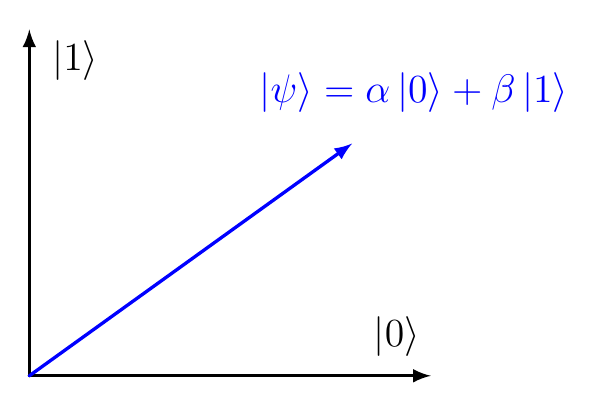
\begin{tikzpicture}[x=1cm,y=1cm,line cap=round,line join=round,>=latex]
        % Axes
        \draw[black,very thick,->] (0,0) -- (0,4.4);
        \draw[black,very thick,->] (0,0) -- (5.1,0);

        % State vector
        \draw[blue,very thick,->] (0,0) -- (4.1,2.95);

        % Labels
        \node[anchor=west,font=\Large] at (2.8,3.6) {\textcolor{blue}{$\ket{\psi} = \alpha \ket{0} + \beta \ket{1}$}};

        \node[anchor=east,font=\Large] at (1.0,4.0) {$\ket{1}$};
        \node[anchor=west,font=\Large] at (4.25,0.5) {$\ket{0}$};
        \end{tikzpicture}
      }}
    \end{column}
  \end{columns}
\end{frame}

\begin{frame}{Probability and dot product}
      \begin{itemize}[<+->]
        \setlength{\itemsep}{0.6em}
        \item Dot product between two quantum states: $\braket{\phi}{\psi}$\\~\\
        \item It translates into a dot product between their associated vectors:\\
         $$\ket \psi = \begin{pmatrix} \alpha \\ \beta \end{pmatrix},\quad  \ket \phi = \begin{pmatrix} \gamma \\ \delta \end{pmatrix} \qquad \braket{\phi}{\psi} =  \gamma^*\alpha + \delta^*\beta$$\\~\\
        \item Examples: $\qquad \braket{0}{0} = 1, \qquad \braket{0}{1} = 0, \qquad \braket{1}{1} = 1$\\~\\
        \item The probability of obtaining a measurement result $\ket  0$ or $\ket 1$ is computed from the dot product between $\ket \psi$ and $\ket 0$ or $\ket 1$:
        $$ |\braket{0}{\psi}|^2 = |\alpha|^2, \qquad  |\braket{1}{\psi}|^2 = |\beta|^2$$
      \end{itemize}
\end{frame}


\begin{frame}{End of chapter 2}
  \begin{enumerate}
    \item Vectors\\~\\
    %\item Dot product\\~\\
    \item Qubit, superposition of states and vectors\\~\\
    \item Mesure de l'état d'un qubit
  \end{enumerate}
\end{frame}

\end{document}
